\documentclass{article} % for short documents
%\documentclass{report} % for longer documents

\usepackage{minted}

%% Defining the language for the document
\usepackage[english]{babel}
\usepackage[english]{isodate}

\usepackage{imta_core}
\usepackage{imta_extra}
\usepackage{epigraph}
\usepackage{graphicx}
\usepackage{wrapfig}
\usepackage{alertmessage}
\usepackage{hyperref}
\usepackage{xcolor}


%% Addtionnal packages can be loaded here
% \usepackage{biblatex} % for a complete and flexible bibliography


\cleanlookdateon % formats date according to the loaded language from now on

%% General informations
\author{\\ Alexandre ALLANI \\
	Adrien CLOTTEAU }
%\imtaAuthorShort{<author's initials>}
%\imtaSuperviser{<superviser>}
\date{\noexpand\today} % automatically print today's date, can be redefined using \date{<date>}
\title{Rapport projet S5}
\subtitle{Challenge Total}
%\imtaVersion{<version>}

%Add extra other companies' logo
%If needed, options can be passed to the underlying \includegraphics by calling \imtaAddPartnerLogo[<options>]{<path>}
%\imtaAddPartnerLogo{<logo_path>}


\imtaSetIMTStyle % Sets font and headers/footers according to the IMT Atlantue style guidelines

%%%%%%%%%%%%%%%%%%%%%%%%%%%%%%% 
%%%%%%%%%% BEGINNING %%%%%%%%%% 
\begin{document}
	
	% front cover
\imtaMaketitlepage
\tableofcontents
\newpage

\section{Introduction}
\alertinfo{Vous trouverez l'ensemble de ce qui a été fait en suivant le lien ci-dessous. \url{https://github.com/Syndorik/ChallengeTotal}. 
}
En suivant le lien Github, vous trouverez: 
\begin{itemize}
	\item Challenge-Total-Overlook-of-the-data.ipynb : Jupyter Notebook sur la visualisation des donnés
	\item Data Engineering and Modeling.ipynb : Jupyter Notebook sur la préparation des données et la modélisation
	\item Time\_series.ipynb : Jupyter Notebook sur la modelisation avec les Time Series.
\end{itemize}
\section{Contexte}
\newpage
\section{Visualisation des données}
\alertinfo{Le code lié à cette partie est disponible sur le lien suivant \url{https://github.com/Syndorik/ChallengeTotal/blob/master/Challenge-Total-Overlook-of-the-data.ipynb}. 
}
\newpage
\section{Préparation des données (Data Engineering)}
\alertinfo{Le code lié à cette partie est disponible sur le lien suivant \url{https://github.com/Syndorik/ChallengeTotal/blob/master/Data-Engineering-and_Modeling.ipynb}. 
}
Dans cette partie, nous allons présenter la préparation des données faites avant les dernières modélisation. En suivant la méthodologie CRISP, cette préparation des données est le fruit de plusieurs tests/modélisation. Nous ne présenterons que les résultats fructueux, qui ont mené à une amélioration du modèle.
\subparagraph{Modification du jeu de données}
Le jeu de données étant Français et l'interpréteur utilisé étant sous le format anglo-saxon, les valeurs numériques (tels que la température, la nébulosité etc.) étaient considérés comme des chaînes de cratère à cause de la virgule. Nous avons donc remplacé les "," par des "." pour pallier à ce problème.\\
Par ailleurs, le jeu de donnée ne contenant aucune valeur non acquises (NA values), il n'y a pas eu de pré-traitement à faire.

\subsection{Segmentation temporelle}
\subsubsection{Distinction des vacances}
L'une des premières améliorations effectuée au niveau des données est la segmentation du jeu de données en période de vacances et période de "travail". En effet, il est important de modéliser cette saisonnalité car les ventes sont très différentes pendant et hors des périodes de vacances. 
\begin{figure}[!h]
	\centering
	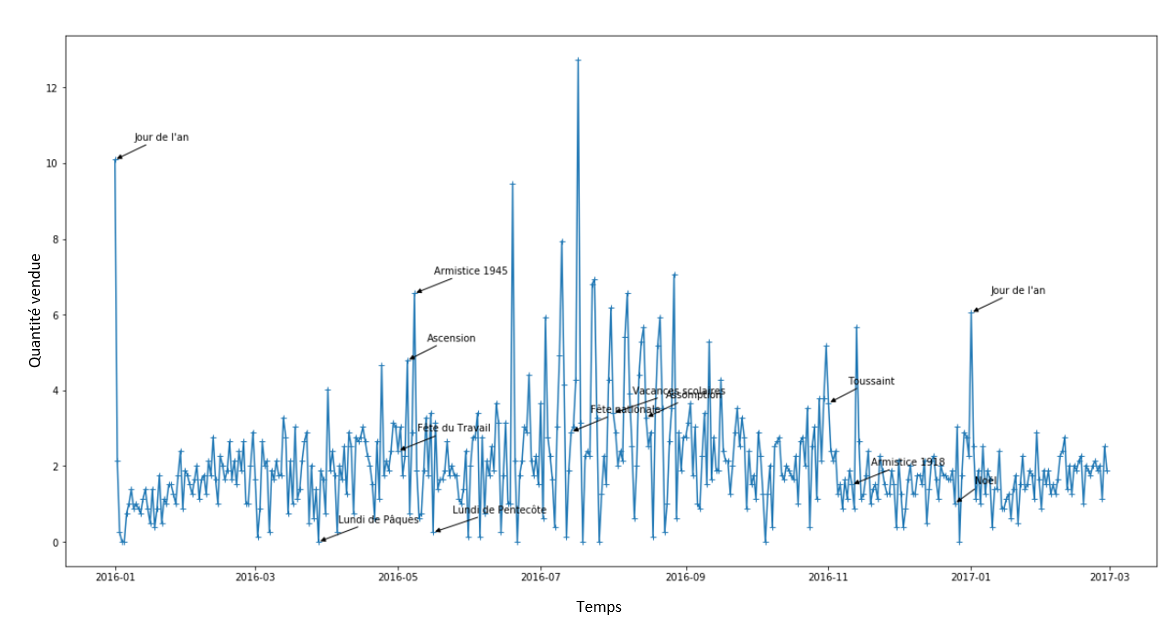
\includegraphics[keepaspectratio = true,scale=0.65]{varvente.png}
	\caption{Vente de baguette au cours de la période}
	\label{bbg}
\end{figure}
Le graphique ci-dessus, \textbf{Figure ~\ref{bbg}} représente les ventes des baguettes sur les deux stations durant la période couverte par le jeu de données. Les baguettes sont le produit le plus vendus, tout produits confondus. Nous pouvons observer que les ventes lors des jours fériés et périodes de vacances sont beaucoup plus grandes. En particulier, les grandes vacances sont plus sujettes à de fortes variations.\\
Ces observations sont logiques, les périodes de vacances correspondes aux périodes de départs. Les familles vont en général plus s'arrêter dans les stations services, ainsi la quantité de produit vendu est beaucoup plus grande.\\
Segmenter l'année permet de mettre en évidence les périodes où les ventes sont très variables par rapport à la moyenne et donc permet d'affiner notre modèle.En se basant sur les \href{https://vacances-scolaires.education/annee-2015-2016.php}{\underline{\textbf{\textcolor[rgb]{0,0,1}{vacances 2015-2016}}}} et les \href{https://vacances-scolaires.education/annee-2016-2017.php}{\underline{\textbf{\textcolor[rgb]{0,0,1}{vacances 2016-2017}}}}, nous avons pu segmenter la période selon les vacances scolaires et les zones de départ en créant une nouvelle variable "holidays".
\begin{figure}[!h]
	\centering
	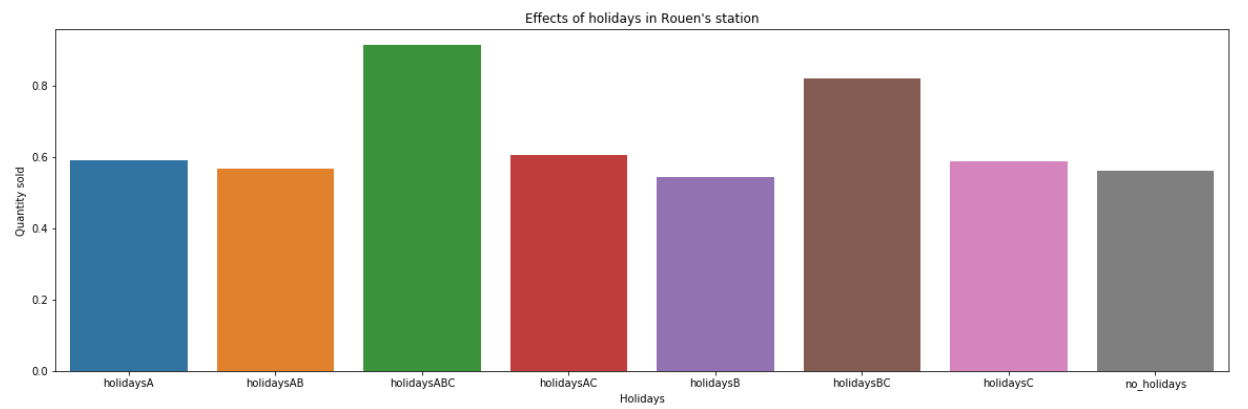
\includegraphics[keepaspectratio = true,scale=0.65]{saleholiday.png}
	\caption{Vente cumulé par semaine selon la journée}
	\label{fig:salehol}
\end{figure}
~\\
Après création de ces variables, nous pouvons comparer les ventes moyennes entre les différentes périodes de vacances grâce à la \textbf{Figure ~\ref{fig:salehol}}. Il apparait qu'il y a une réelle différence lorsque toutes les zones (A, B, C) sont en vacances ou juste les zones (B,C). Dans les autres cas, il n'y a pas beaucoup de différence avec les périodes de travails. Cela s'explique par le fait que les stations situés à Rouen sont en zone B, et la plupart des voyageurs se dirigeants vers Rouen doivent passer par Paris (zone C). Ainsi lorsque les deux zones sont en vacances en même temps, il y a bien plus d'aller-retour qu'en période normale. Nous choisissons de garder la discrimination entre les vacances pour les trois zones (A,B,C), les vacances pour les zones B et C, et finalement les périodes de "travail".
\subsubsection{Distinction des dates de départs}
Nous pouvons voir sur la \textbf{Figure ~\ref{bbg}} que les premières journées et dernières journées de vacances sont particulièrement haut en terme de quantité vendue. Cela n'est pas surprenant, ce sont des journées où beaucoup de famille sont sur les routes, ainsi il y a mécaniquement plus de ventes qui sont effectuées.\\
Il est donc intéressant de discriminer ces journées afin de mieux les modéliser. Pour cela nous avons créer une nouvelle variable "departure"  qui segmente le jeu de donnée selon les dates de départs.

\subsubsection{Segmentation de la période selon les journées et mois}
Dans l'optique d'exploiter au maximum les saisonnalités des ventes, nous avons continué à travailler sur les dates. Comme nous pouvons le remarquer sur la \textbf{Figure ~\ref{bbg}}, les ventes atteignent un maximum local de manière périodique environ tout les 7 jours. Il y a une périodicité remarquable au niveau de la semaine. En effet, le trajet Paris Rouen ne dure que 2 heures, il est envisageable que certaines personnes font l'aller-retour chaque semaine pour rentrer le week-end, et donc s'arrêtent aux deux stations services.\\
\begin{figure}[!h]
	\centering
	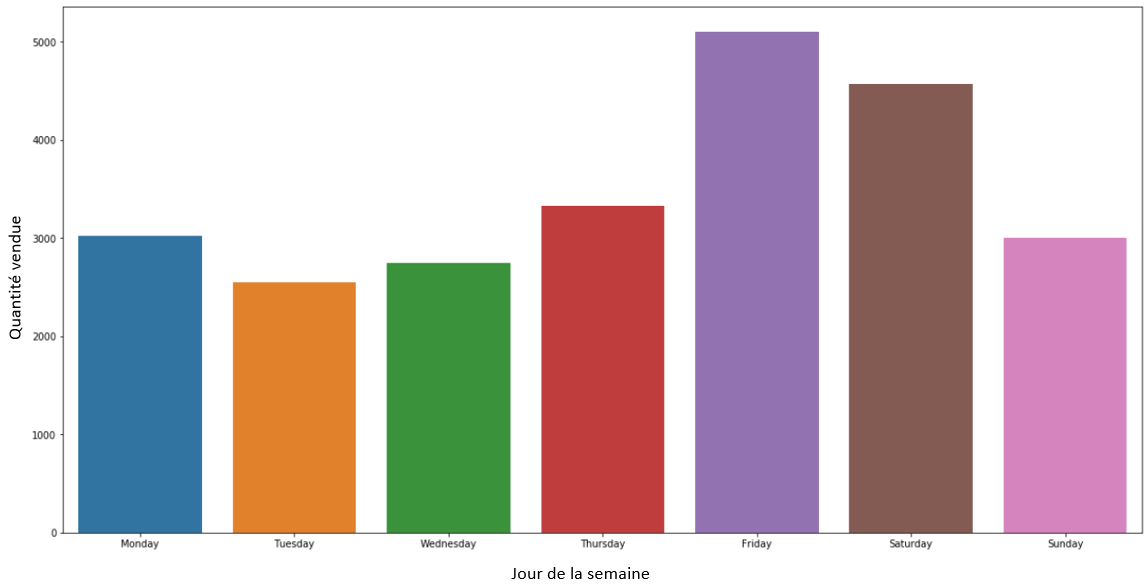
\includegraphics[keepaspectratio = true,scale=0.65]{vente_week.png}
	\caption{Vente cumulé par semaine selon la journée}
	\label{bb1}
\end{figure}
~\\
La \textbf{Figure ~\ref{bb1}} représente le nombre de vente cumulé sur la période du jeu de donnée en fonction des jours de la semaine. Elle met en évidence cette périodicité. Les ventes des journées du Vendredi et Samedi sont bien au dessus des autres jours de la semaine. De manière générale, les ventes sont faibles pendant la semaine et haute pendant le week-end. C'est pourquoi nous avons différencié chaque jour de la semaine dans notre jeu de données.\\
\subsubsection{Suppression de la colonne date}
Une fois ces transformations réalisés, nous supprimons la colonne date. En effet pour les modèles que nous allons utilisé (excepté pour les Time Series), garder les dates va entraîner du sur-apprentissage. Les modèles vont apprendre sur la date exacte (jour-mois-année), sachant que ces dates sont passés, cela va entraîner une grande erreur.\\
Il est à noter que toutes ces segmentations temporelles ont pour but d'affiner le modèle, et retirer le plus d'information de la variable \textit{date}. Cependant pour le modèle basé sur les Time Series l'ensemble de ces segmentations ne seront pas conservés, car incompatible avec le modèle. Nous expliciterons plus ce sujet dans la \textbf{section ~\ref{sec:tm}}

\subsection{Influence des catégories}
Nous voulions savoir si la distinctions par catégorie était utile, sachant qu'il y a inclusion des catégories : $cat6 \subset cat5 \subset cat4$. La \textbf{Figure ~\ref{cat5p1} et ~\ref{cat5p2} } représente les ventes en fonction de la catégorie 5 pendant la période.\\ 
\begin{figure}[!h]
	\centering
	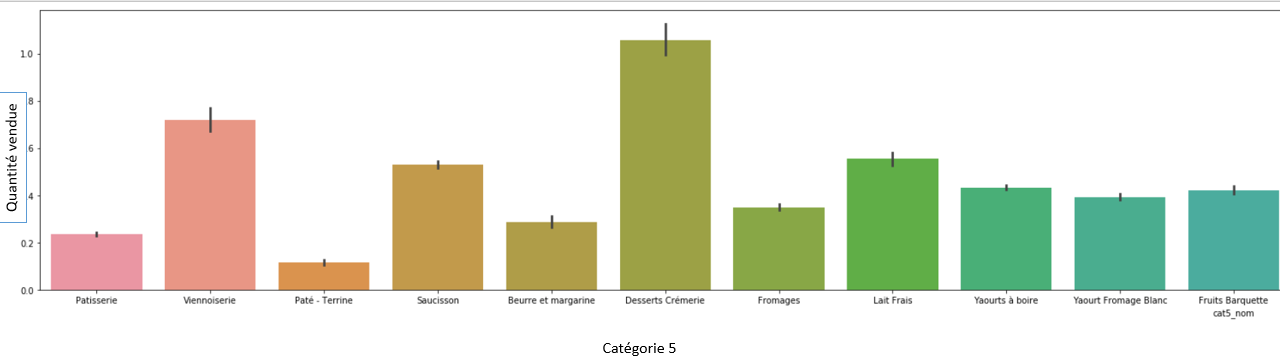
\includegraphics[keepaspectratio = true,scale=0.65]{categorie5part1.png}
	\caption{Vente cumulé en fonction de la catégorie 5 (partie 1)}
	\label{fig:cat5p1}
\end{figure}
~\\
Il est clair qu'il y a une différence de vente en fonction de la catégorie. La catégorie \textit{Sandwich} ou encore \textit{Dessert Crémerie} domine, tandis que la catégorie \textit{pâté} et \textit{autre charcuterie} font de faibles ventes. Cependant comme  on peut le voir sur la \textbf{Figure ~\ref{bb3}} (Annexe ~\ref{sec:catprod}), il y a peu de différence entre les sous catégories, en particulier entre la catégorie 5 et 6 qui paraissent être presque les mêmes. Cela s'explique par l'inclusion des catégories.\\
En réalisant les tests de modélisation, nous avons supprimé la catégorie 5 pour éviter la redondance des données, ce qui n'a pas affecté nos modèles. Ainsi on conservait le regroupement par catégorie qui permet d'avoir une version plus grossière de nos produit, et un certain clustering, tout en limitant le nombre de variables pour éviter le \textit{Fléau de la dimension} (\textit{"curse of dimensionality"}). 
\begin{figure}[!h]
	\centering
	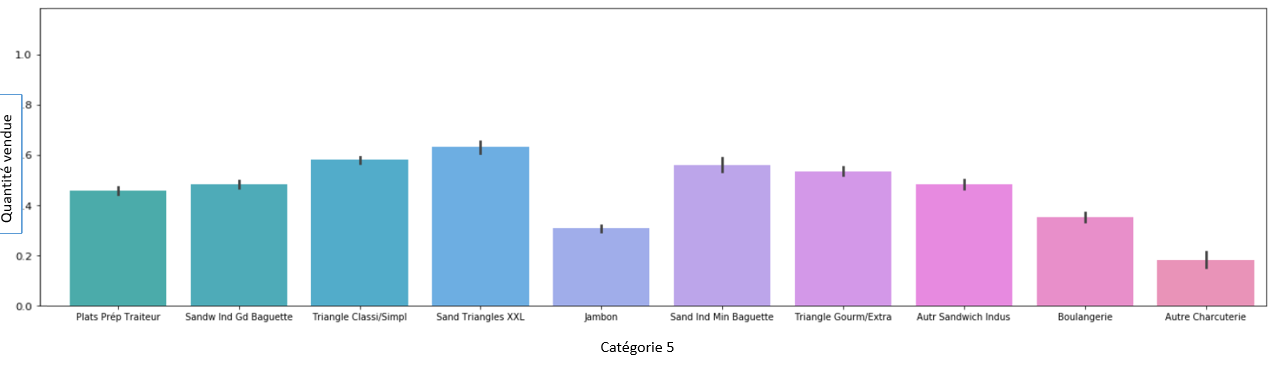
\includegraphics[keepaspectratio = true,scale=0.65]{categorie5part2.png}
	\caption{Vente cumulé en fonction de la catégorie 5 (partie 2)}
	\label{fig:cat5p2}
\end{figure}
\subsection{Transformation des données}
\subsubsection{One Hot Encoding}
Le One Hot Encoding est une transformation des données catégoriel en vecteur binaire. La \textbf{Figure ~\ref{fig:OHE}} représente une telle transformation.
\begin{figure}[!h]
	\centering
	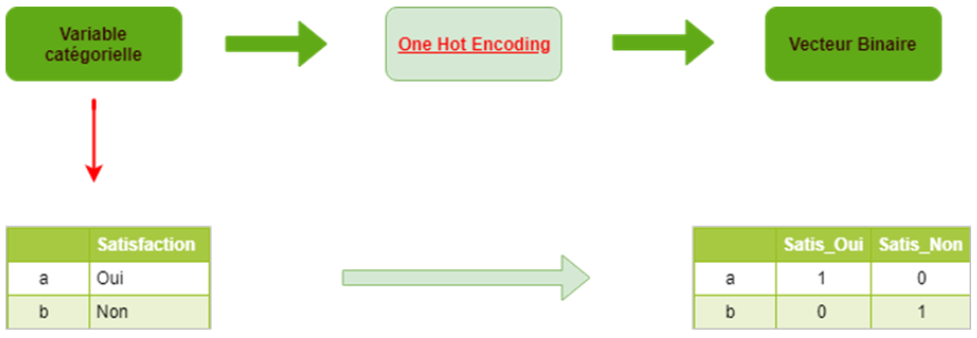
\includegraphics[keepaspectratio = true,scale=0.55]{OHE.png}
	\caption{Principe du One Hot Encoding}
	\label{fig:OHE}
\end{figure}
Le principe est de créer un ensemble de nouvelles variables représentant une variables catégorielle (une variable par possibilité différente) prenant des valeurs binaires (0 ou 1). Il est important de faire cette transformation car plusieurs algorithme de machine learning n'arrivent pas à travailler avec les variables catégorielles. En l'occurrence, concernant notre projet les modèles suivants ne supportent pas les variables catégorielles: \begin{itemize}
	\item Modèle linéaire
	\item Réseau de Neurone
\end{itemize}
Cependant il y a plusieurs désavantage à cette technique:
\begin{itemize}
	\item L'augmentation du nombre de dimensions qui est la cause de la \textit{"curse of dimensionality"}. Le traitement de donnée devient plus difficile et long, car les données prennent plus de place en mémoire
	\item Les éléments du vecteurs sont équidistant, impliquant que chaque modalité d'une variable catégorielle ait la même importance ce qui n'est pas le cas. (Par exemple, le fait qu'il y a des vacances en zone A, B et C est plus important que le fait qu'il n'y ait pas de vacances)
	\item Le vecteur binaire ne contient une information sémantique encodée, ce qui rend plus difficile la compréhension.
\end{itemize}
Cette méthode étant simple à appliquer et permettant l'utilisation direct de la majorité des algorithme, nous allons tout de même l'utiliser dans la suite du projet.
 
\subsubsection{Normalisation des données}


\newpage
\section{Modélisation}
\subsection{Modélisation basée sur le Data Engineering}

\alertinfo{Le code lié à cette partie est disponible sur le lien suivant \url{https://github.com/Syndorik/ChallengeTotal/blob/master/Data-Engineering-and_Modeling.ipynb}. 
}

\subsection{Modélisation basée sur les Time Series}
\label{sec:tm}
\alertinfo{Le code lié à cette partie est disponible sur le lien suivant \url{https://github.com/Syndorik/ChallengeTotal/blob/master/Time_series.ipynb}. 
}

\newpage
\section{Analyse des résultats}

\newpage
\section{Conclusion}

\newpage
\section{Annexe}
\subsection{Vente par Catégorie de produit}
\label{sec:catprod}
\begin{figure}[!h]
	\centering
	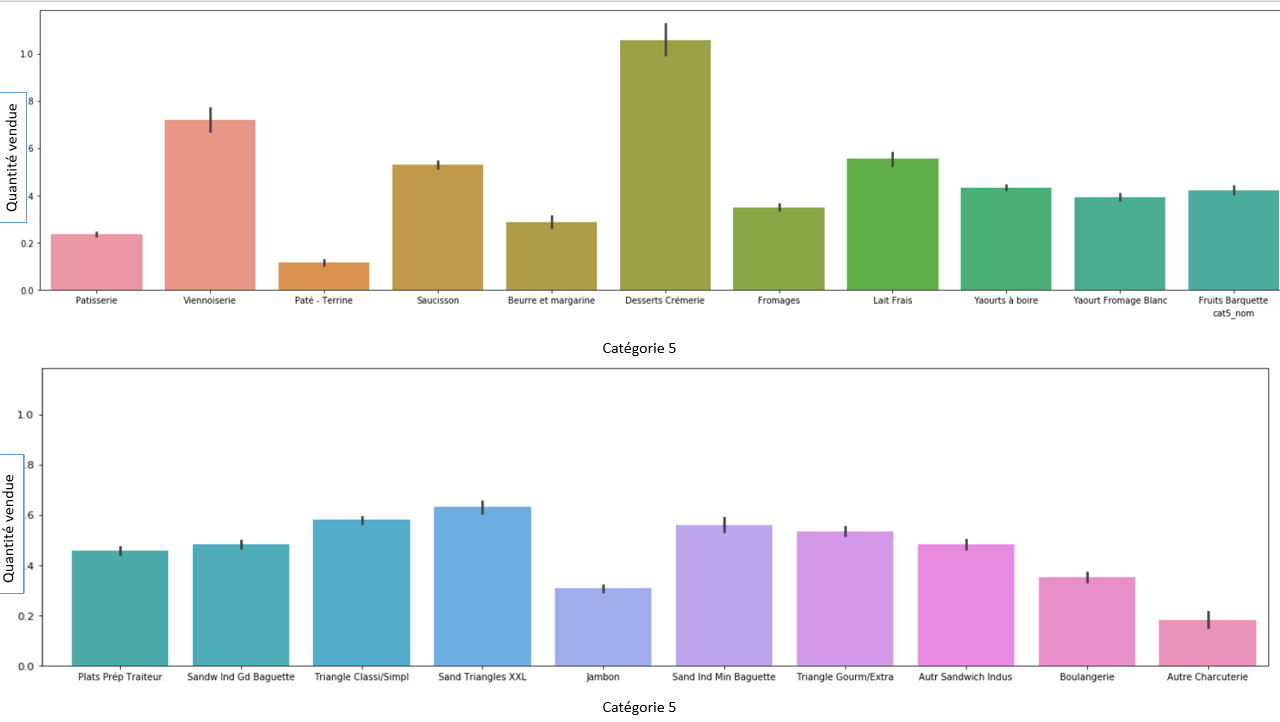
\includegraphics[keepaspectratio = true,scale=0.65]{categorie.png}
	\caption{Vente cumulé en fonction de la catégorie 5}
\end{figure}

\begin{figure}[!h]
	\centering
	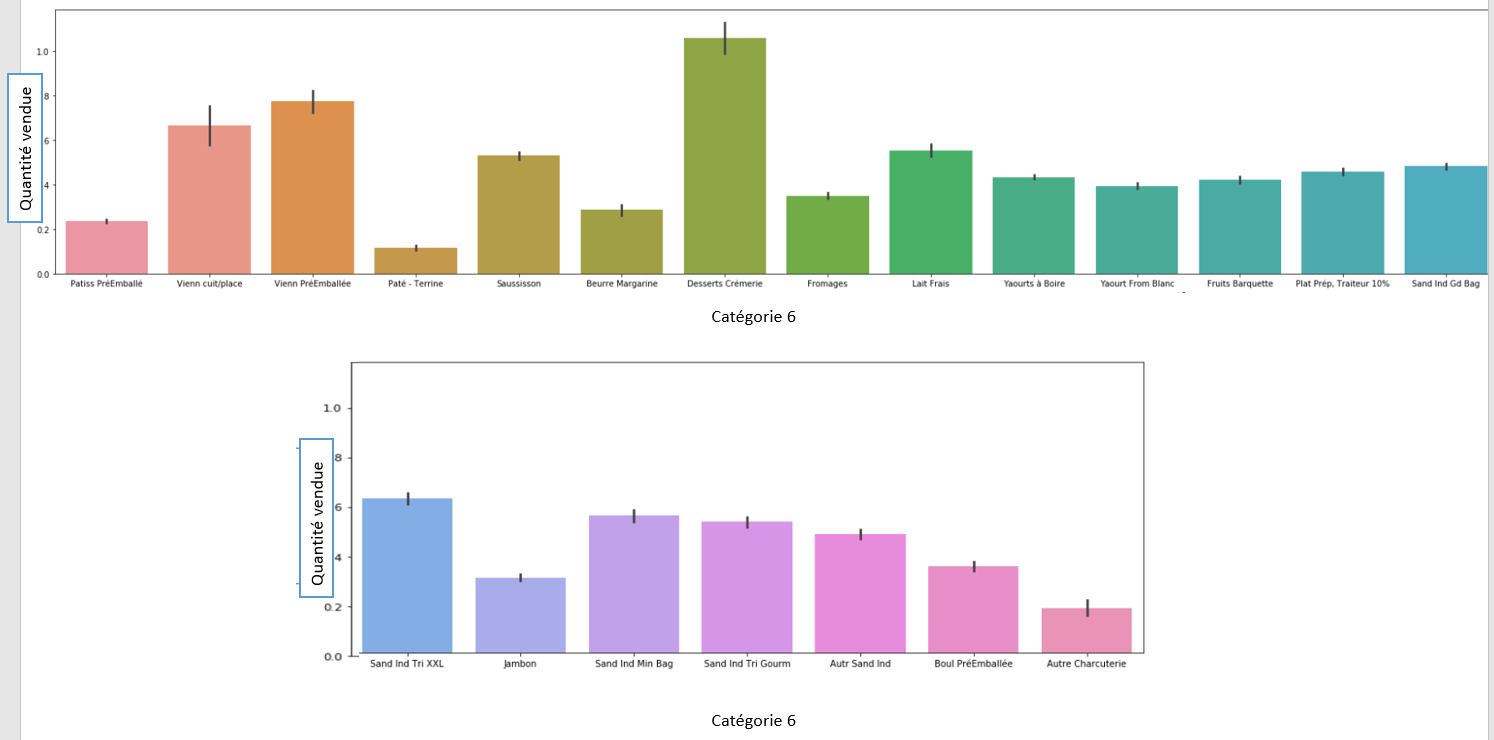
\includegraphics[keepaspectratio = true,scale=0.55]{categorie6.png}
	\caption{Vente cumulé en fonction de la catégorie 6}
	\label{bb3}
\end{figure}
\newpage
\begin{figure}[!h]
	\centering
	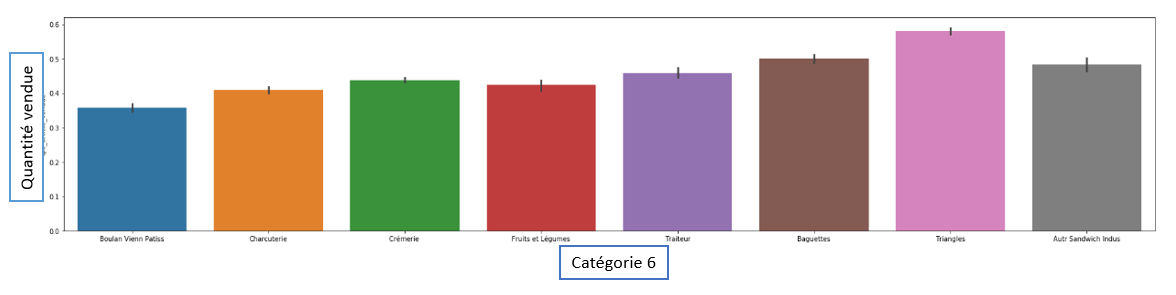
\includegraphics[keepaspectratio = true,scale=0.55]{categorie4.png}
	\caption{Vente cumulé en fonction de la catégorie 4}
	\label{bb3}
\end{figure}
\end{document}
%%%%%%%%%% END %%%%%%%%%% 
%%%%%%%%%%%%%%%%%%%%%%%%% 
